\section{Cerca de persones per localitzacions}

\subsection{Introducció i demostració}

\paragraph{}
Aquest problema és detectat quan obtenim accés a producció i comencem a jugar amb la funcionalitat evolució d'esdeveniments, ja que en l'entorn de producció `sandbox', no era detectable.

La prova pilot d'aquesta funcionalitat, es basava en la cerca a l'arbre familiar, per només la localització de naixement, casament o defunció.

Quan es comencen a realitzar proves en l'entorn de producció, el nombre de resultats retornats per cada any de l'interval, és definitivament més baix del que esperàvem. Per comprendre el que estava passant, vam realitzar una investigació a través de la funcionalitat de cerca, també implementada en la prova pilot.

En la primera cerca de prova, demanem a la funcionalitat cerca de persones, que retorni totes les persones nascudes als Estats Units. Sorprenentment, la cerca només retorna 168.117 resultats (figura~\ref{fig:searchStates}).

\begin{figure}[h]
    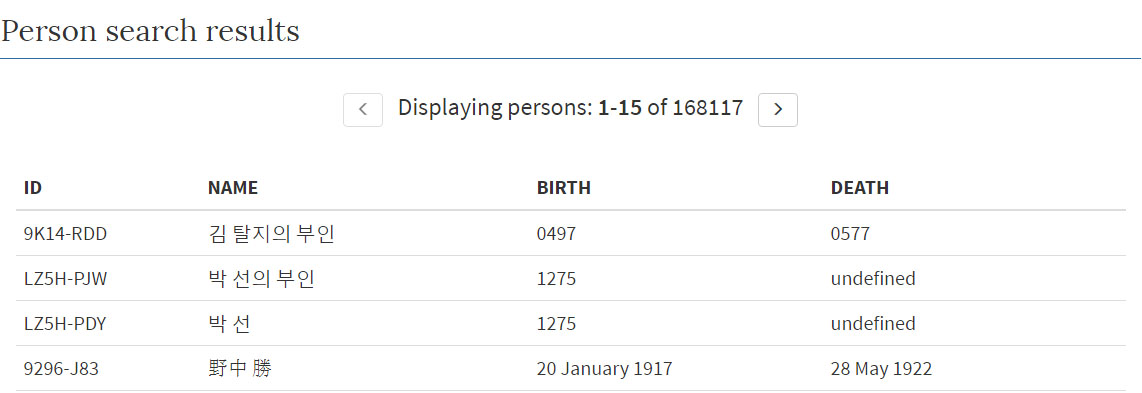
\includegraphics[width=\linewidth]{11.5/00_places}
    \centering
    \caption{Cerca per persones nascudes als Estats Units}\label{fig:searchStates}
\end{figure}

Aquest nombre és evidentment incorrecte, perquè si realitzem una cerca per aquelles persones que es diuen Tom i que a més a més, han nascut als Estats Units, la cerca retorna 2.909.316 persones (figura~\ref{fig:searchTom}). Aquest nombre, que `en principi hauria de ser més petit', que el retornat per la primera cerca, ens indica que alguna cosa no acaba de funcionar, en la cerca del SDK.

\begin{figure}[h]
    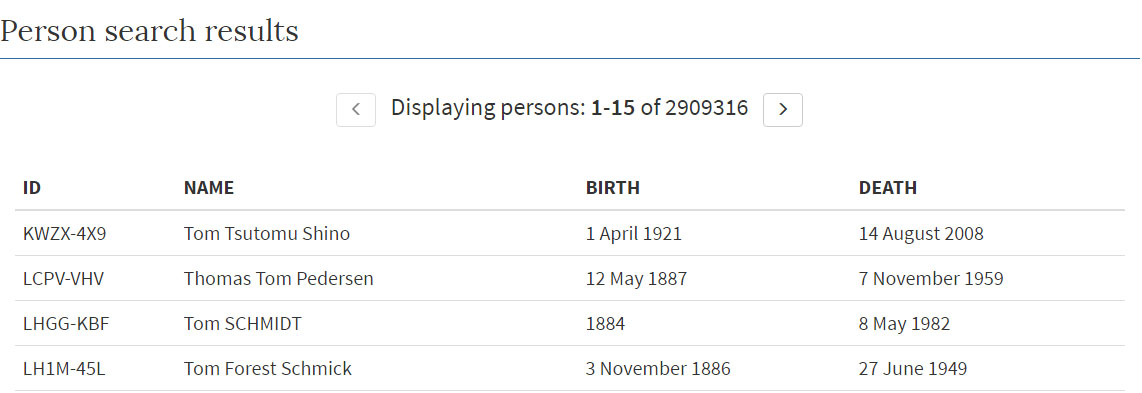
\includegraphics[width=\linewidth]{11.5/01_places}
    \centering
    \caption{Cerca per persones amb nom Tom i nascudes als Estats Units}\label{fig:searchTom}
\end{figure}

Així doncs, si ens fixem en els resultats retornats en la resposta de la primera cerca (figura~\ref{fig:searchStates}), podem observar com tots els resultats retornats semblen contenir caràcters no llatins. En altres paraules, el conjunt de persones retornades sembla estar format per Coreans, Japonesos, Xinesos, etcètera, etcètera.

Aquest fet ens fa sospitar que la funcionalitat de cerca és incapaç de retornar resultats correctes, si no s'especifica algun dels paràmetres \emph{nom} o \emph{cognom}, per la persona cercada o algun dels familiars més propers.

Aquesta hipòtesi es veu reforçada al realitzar més comprovacions. Al final, es pot concloure que el motiu pel qual la primera cerca retornava 168.117 persones, era perquè aquest és el col·lectiu de persones que complia la condició de cerca, en què el nom o cognom no estava format per caràcters llatins o bé estaven buits.


\subsection{Implicacions del problema}

\paragraph{}
El primer que caldria comprovar és si aquest problema també succeeix mitjançant la connexió directa amb l'API de FamilySearch. En cas de ser així, probablement aquest obstacle no seria superable de forma directa i implicaria que la cerca global de persones, a través de la introducció d'una localització de naixement, casament o defunció, no es troba suportada pel sistema.

Aquesta restricció també significa, que almenys, a través del SDK, la funcionalitat d'evolució d'esdeveniments, plantejada en la prova pilot, no acabaria de funcionar i caldria trobar mètodes alternatius, per tal de poder produir gràfics basats en una quantitat de dades més elevada.

Per exemple, realitzar la cerca pels noms o cognoms més comuns del país introduït i agregar les dades o realitzar directament la cerca, per una localització i cognom especificats per l'usuari, en comptés de només una localització.

El que està clar, és que és una restricció a tenir en compte de cara a la rea\-lit\-za\-ció de futurs projectes, si és que es confirma que aquest problema també succeeix mitjançant la connexió directa a l'API.

De totes maneres, sempre existeixen alternatives que poden permetre afrontar les tasques de forma indirecta i aquest problema s'ha fet latent a l'organització Family\-Search, a través del grup per desenvolupadors de Google, amb l'esperança de què pugui ser adreçat en un futur.
